\section{Auswertung}
\subsection{Photolumineszenz-Eigenschaften der kolloidalen Nanokristalle}
Die erste Aufgabe ist es, einige Eigenschaften der kolloidalen Nanokristalle anhand von Photolumineszsenzspektren zu untersuchen.
\subsubsection{ Gr\"{o}{\ss}e der Nanokristalle}
Zun\"{a}chst soll die Gr\"{o}{\ss}e der kolloidalen Nanokristalle jeder Probe bestimmt werden.
Hierf\"{u}r wird jede Probe einzeln mit einem Laser der Wellenl\"{a}nge $405 \,$nm angeregt und ein Photolumineszsenzspektrum (PL-Spektrum) von ca $320$ - $747 \,$nm wird aufgenommen.
Diese PL-Spektren sind in Abbildung (\ref{abb:auf1a}) zu sehen. 
\begin{figure}[H]
\centering
	\begin{subfigure}[t]{0.4\textwidth}
	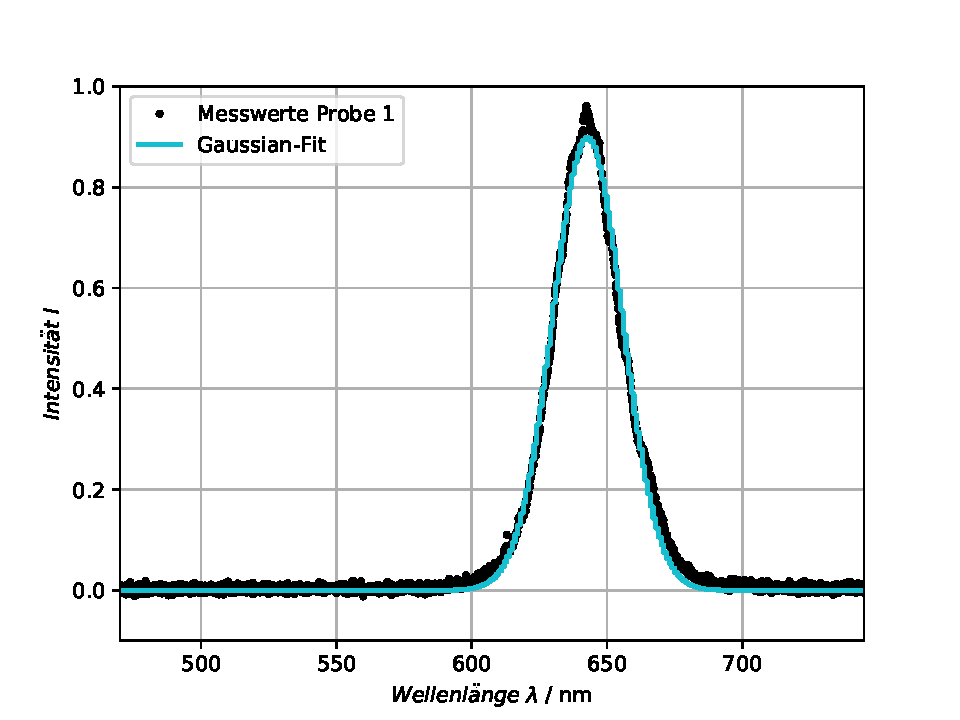
\includegraphics[width=\textwidth]{Plots/aufgabe1a_P1.pdf}
	\caption{Messung der Probe 1 mit Messdauer $1 \,$s.}
	\label{abb:A1_P1}
	\end{subfigure}
	~
	\begin{subfigure}[t]{0.4\textwidth}
	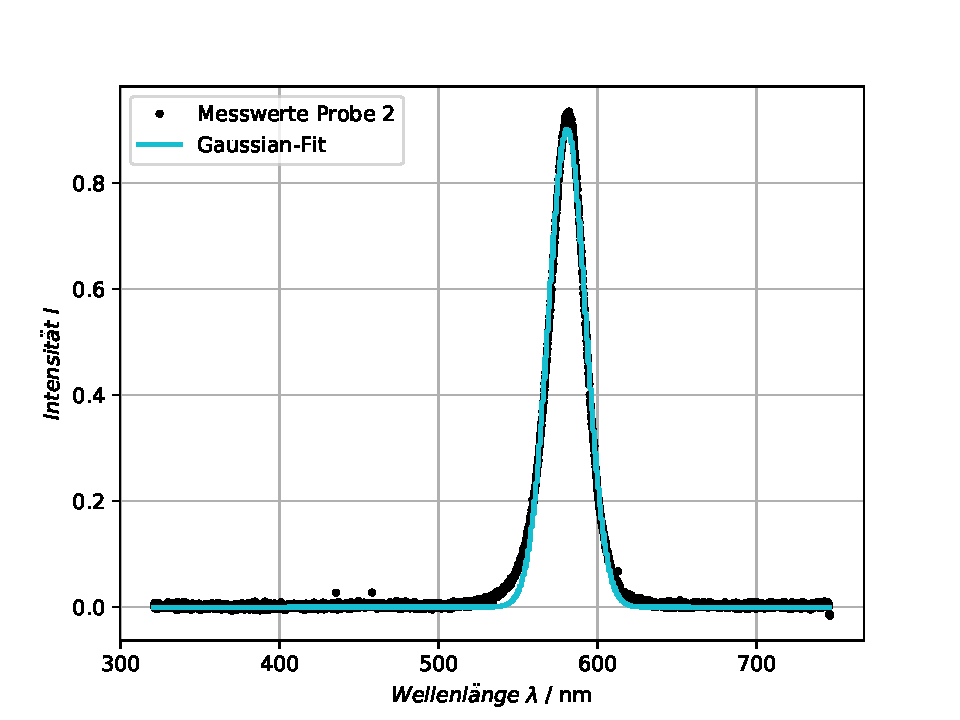
\includegraphics[width=\textwidth]{Plots/aufgabe1a_P2.pdf}
	\caption{Messung der Probe 2 mit Messdauer $0,5 \,$s.}
	\label{abb:A1_P2}
	\end{subfigure}
	~
	\begin{subfigure}[t]{0.4\textwidth}
	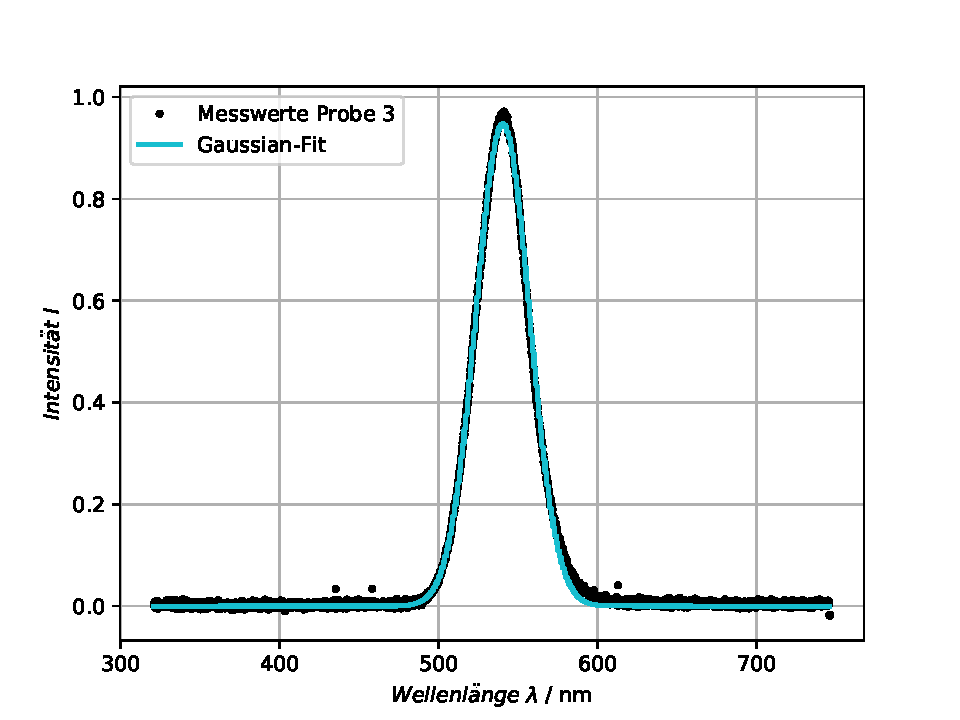
\includegraphics[width=\textwidth]{Plots/aufgabe1a_P3.pdf}
	\caption{Messung der Probe 3 mit Messdauer $0,65 \,$s.}
	\label{abb:A1_P3}
	\end{subfigure}
\caption{Photolumineszsenzspektren der drei vorliegenden Proben mit einer Anregungswellenl\"{a}nge von 405 nm.}
\label{abb:auf1a}
\end{figure}
Mit Hilfe von Magicplot und Python werden durch die Messwerte aller drei PL-Spektren gau{\ss}f\"{o}rmige Ausgleichs{\-}kur{\-}ven gelegt.
Diese besitzen die in Formel (\ref{form:gauss}) beschriebene Form.
\begin{align}
	y = a \cdot exp \left( -ln(2) \cdot \frac{(x-x_0)^2}{dx^2} \right)
\label{form:gauss}
\end{align}
Hierbei gibt $a$ die Amplitude und $dx$ die Linienbreite an.
Die Variable $x_0$ gibt die Wellenl\"{a}nge $\lambda_i$ der Probe an.

Die Messwerte in Abbildung (\ref{abb:A1_P1}) weisen im Unterschied zu den anderen PL-Spektren (Abbildung (\ref{abb:A1_P2}) und (\ref{abb:A1_P3})) Abweichungen im Bereich des Emissionsmaximum auf.
Auff\"{a}llig sind die an der abfallenden Flanke zu sehenden lokalen Maxima.
Die Messwerte des PL-Spektrum der Probe 2 mit einer Emissionswellenl\"{a}nge von $580,83 \,$nm steigen am Anfang der ansteigenden Flanke wesenltisch langsamer an.
Auch hier ist eine Abweichung im Bereich des globalen Maximums zu sehen, diese ist jedoch wesentlich geringer im Verh\"{a}ltnis zur ersten Probe.
Im PL-Spektrum der Probe 3 (siehe Abbildung (\ref{abb:A1_P3})) ist nur eine Abweichung der Gau{\ss}form in der abfallenden Flanke zu beobachten.

Mittels der Formeln (\ref{form:energie}) und (\ref{form:radius}) lassen sich nun die Gr\"{o}{\ss}e der Nanopartikel berechnen.
\begin{align}
	E_{r,i} &= h \frac{c}{\lambda_i} \label{form:energie}
\end{align}
Alle experimentellen Ergebnisse sind in Tabelle (\ref{tab:auf1a}) aufgelistet.
\begin{table}
	\centering
	\caption{Ergebnisse aus den Fit-Kurven der drei Messungen.}
\begin{tabular}{|r|ccc|}
	\hline
	{Probe} & {Wellenl\"{a}nge $\lambda_i$ / nm} & {Energie $E_{r,i}$ / eV} & {Radius $r_{NP}$ / nm} \\
	\hline
	1	& 642,81(9) &	1,92(89)	&	7,7(17)	\\
	2	& 580,83(2) &	2,13(48)	&	5,3(38)	\\
	3	& 540,28(7) &	2,29(49)	&	4,5(02)	\\
	\hline
\end{tabular}
\label{tab:auf1a}
\end{table}

\subsubsection{Polarisation der Photolumineszenz}
Im n\"{a}chsten Schritt wird an einer Probe beispielhaft untersucht, ob die Photolumineszsenz polarisiert ist.
In Abbildung (\ref{abb:polarisation}) sind die drei verschiedenen PL-Spektren der Probe drei zu sehen.
\begin{figure}[H]
\centering
	\begin{subfigure}[t]{0.4\textwidth}
	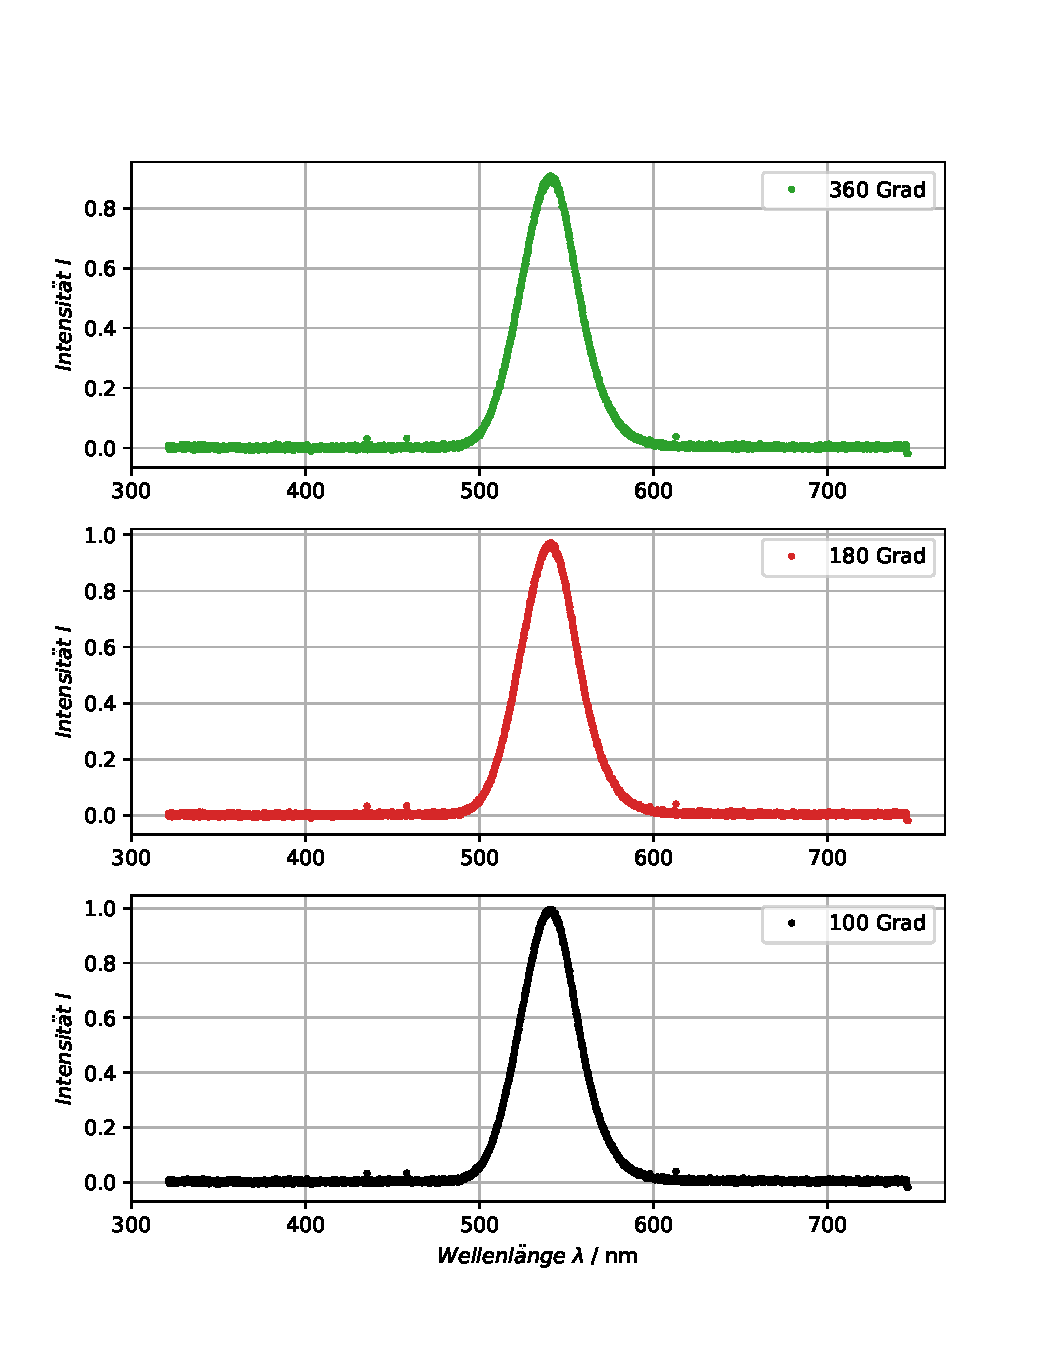
\includegraphics[width=\textwidth]{Plots/aufgabe1b_korrek.pdf}
	\caption{Die drei Messungen einzelnd.}
	\label{abb:polarisation_einzelnd}
	\end{subfigure}
	~
	\begin{subfigure}[t]{0.4\textwidth}
	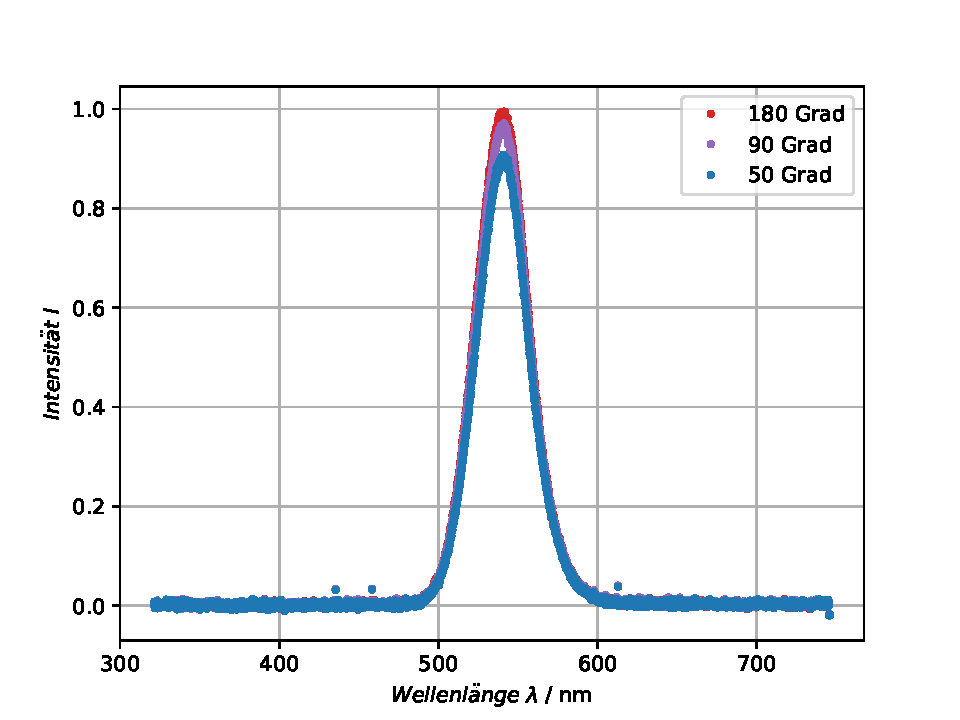
\includegraphics[width=\textwidth]{Plots/aufgabe1b.pdf}
	\caption{Alle Messungen Im Vergleich.}
	\label{abb:polarisation}
	\end{subfigure}
\caption{PL-Spektren der Probe 3 mit einer Anregungswellenl\"{a}nge von $405 \,$nm f\"{u}r drei unterschiedliche Polarisationswinkel im Detektionspfad.}
%\label{•}
\end{figure}
In Abbildung (\ref{abb:polarisation_einzelnd}) ist zu erkennen, dass f\"{u}r verschiedene Polarisationswinkel in der Detektion das Spektrum der Photoluminezsenz dieselbe Form aufweist.
Auch der PL-Peak befindet sich bei allen drei Messungen an ungef\"{a}hr dergleichen Stelle.
Im direkten Vergleich der Messungen, welcher in Abbildung (\ref{abb:polarisation}) dargestellt ist, ist zu erkennen, dass lediglich die Intensit\"{a}t des Peaks ein wenig variiert.
Die Photoluminezsenz h\"{a}ngt somit nicht von der Polarisation des anregenden Lichtes ab.

\subsubsection{Leistungsabh\"{a}ngige Peak-Energie}
Als letzte Eigenschaft wird die Peak-Energie in Abh\"{a}ngigkeit der Leistung untersucht.
Auch diese Messung wird wieder an der Probe 3 durchgef\"{u}hrt.
F\"{u}r sieben verschiedenen Laserleistungen wird das PL-Spektrum aufgenommen.
Um keine S\"{a}ttigung des Detektors zu erreichen, wird die Messzeit f\"{u}r jede Laserleistung variiert.
In Tabelle (\ref{tab:1c}) sind die Messwerte zu den Spektren notiert.
\begin{table}
	\centering
	\caption{Aufgenommene Werte der Messungen zur Leistungsabh\"{a}ngige Peak-Intensit\"{a}t. Sowie die Intensit\"{a}ten nomiert auf $1 \, $s. }
%\begin{tabular}{|D{.}{,}{-1}cc|}
\begin{tabular}{|cccc|}
	\hline
	{Laserleistung / mW} & {Intensit\"{a}t} & {Zeitintervall $\Delta t$ / ms} & {normirte Intensit\"{a}t} \\
	\hline
	0,1	&	0,3311	&	1800 & 0.184 \\
	0,5	&	0,8477	&	1200 & 0.706 \\
	1	&	0,9658	&	700	& 1.380 \\
	5	&	0,9684	&	150	& 6.456 \\
	10	&	0,9286	&	70	& 13.266 \\
	15	&	0,9687	&	50	& 19.374 \\
	20	&	0,7922	&	30	& 26.407 \\
	\hline
\end{tabular}
\label{tab:1c}
\end{table}
Die aufgenommenen PL-Spektren werden mit Formel (\ref{form:gauss}) gefittet.
Um sie untereinander besser vergleichen zu k\"{o}nnen werden die PL-Spektren f\"{u}r eine Messzeit von $1 \, s$ umgerechnet.
In Abbildung (\ref{abb:verLeistung2}) sind diese Kurven zu sehen.
\begin{figure}[H]
\centering
	\begin{subfigure}[t]{0.45\textwidth}
	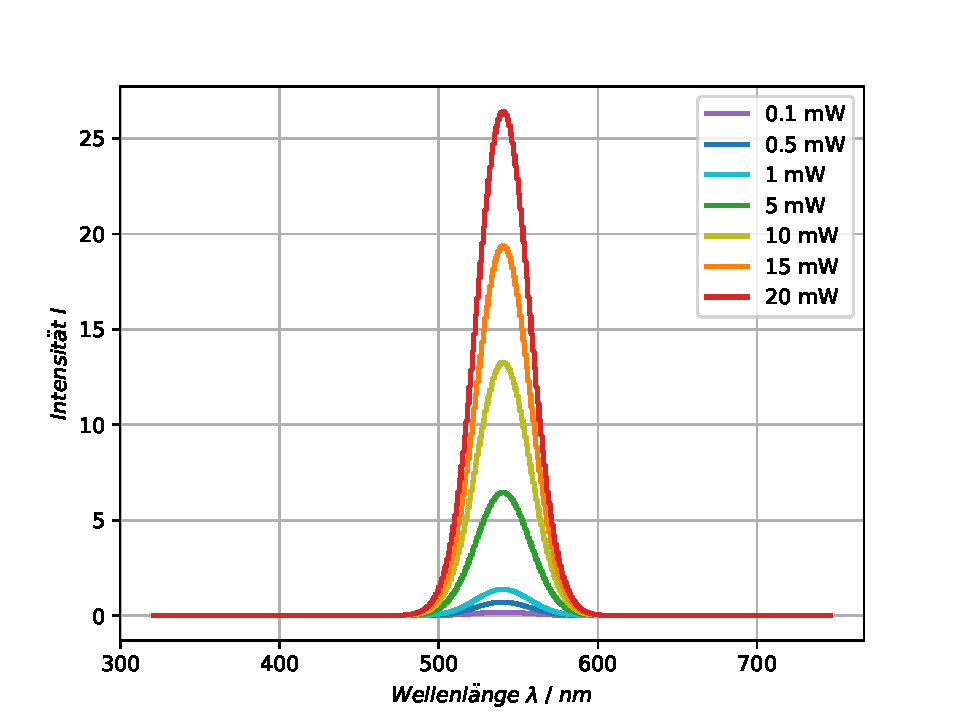
\includegraphics[width=\textwidth]{Plots/aufgabe1c2_1s.pdf}
	\caption{Die Fit-Kurven zu den aufgenommenen PL-Spektren f\"{u}r verschiedenen Laserleistungen mit einer Messzeit von $1$ s.}
	\label{abb:verLeistung2}
	\end{subfigure}
	~
	\begin{subfigure}[t]{0.45\textwidth}
	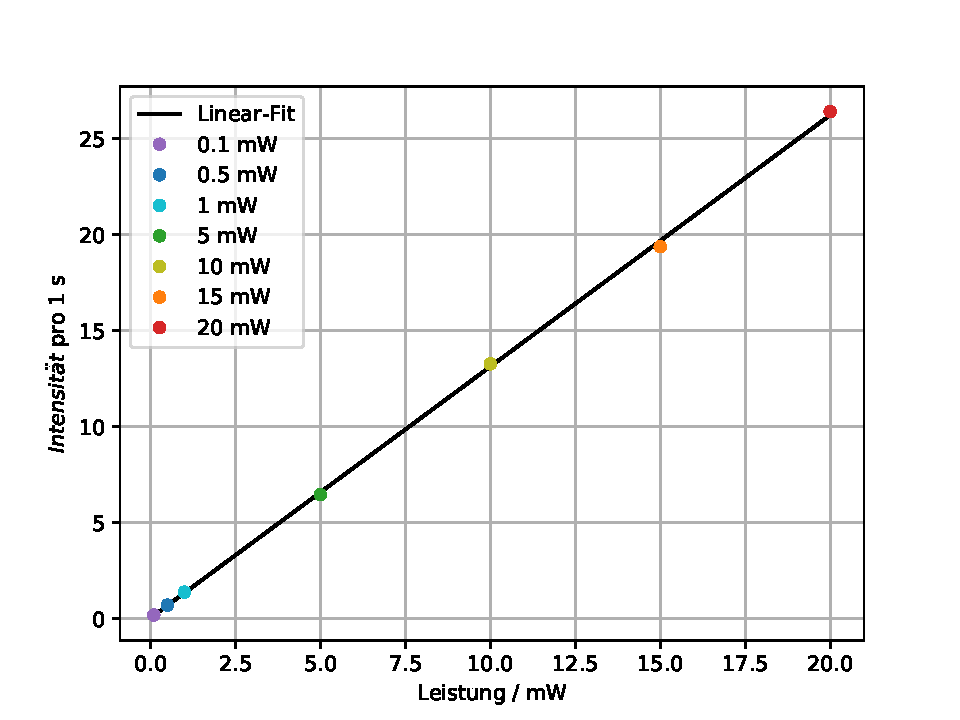
\includegraphics[width=\textwidth]{Plots/aufgabe1c3.pdf}
	\caption{Die Peak-Intensit\"{a}ten der PL-Spektren mit linearem Fit.}
	\label{abb:Leistungen_fit}
	\end{subfigure}
\caption{Messung der Peak-Intensit\"{a}t der Probe 3 mit einer Anregungswellenl\"{a}nge von $405 \,$nm f\"{u}r unterschiedliche Laserleistungen.}
\label{abb:auf1c}
\end{figure}
In Abbildung (\ref{abb:Leistungen_fit}) sind die Peakmaxima gegen die normierte Intensit\"{a}t aufgetragen.
Der lineare Fit bestizt die Form:
\begin{align}
	I_{Peak} = (1,30995 \pm 0,00932)[(\text{mW})^{-1}] \cdot P_{Laser}[\text{mW}] + (0,02559 \pm 0,09654)
	\label{eq:fit1}
\end{align}

%Mittels Formel (\ref{form:energie}) lassen sich die Emissionsenergien der Peaks bestimmen.
In Tabelle (\ref{tab:1c_2}) sind die Messergebnisse der Fit-Kurven aufgelistet.
\begin{table}
	\centering
	\caption{Ergebnisse der Messung zur leistungsabh\"{a}ngigen Peak-Energie und ihrer Linienbreite f\"{u}r eine Messzeit von $1 \, s$.}
\begin{tabular}{|cccc|}
	\hline
	{Laserleistung / mW}	&	{Emissionswellenl\"{a}nge / nm}	&	{Linienbreite / meV}	&	{Amplitude}	\\
	\hline
	0,1	&	540,44(26)	&	20,21(38)	&	0,184	\\
	0,5	&	540,44(65)	&	19,94(69)	&	0,706	\\
	1	&	540,41(80)	&	19,87(45)	&	1,380	\\
	5	&	540,43(98)	&	19,77(09)	&	6,456	\\
	10	&	540,49(21)	&	19,75(19)	&	13,266	\\
	15	&	540,52(85)	&	19,74(76)	&	19,374	\\
	20	&	540,51(86)	&	19,67(78)	&	26,407	\\
	\hline
	\end{tabular}
\label{tab:1c_2}
\end{table}
Und in Abbildung (\ref{abb:auf1c_ergebnisse}) sind Linienbreite und Emissionswellenl\"{a}nge gegen die angelegte Laserleistung aufgetragen.
\begin{figure}[hbtp]
\centering
%	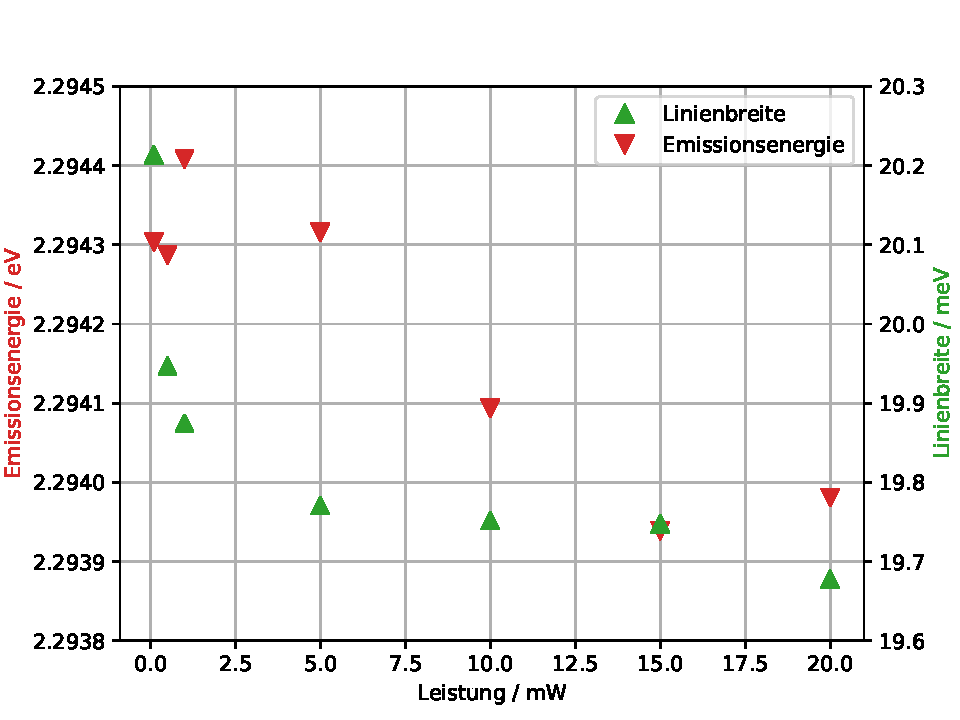
\includegraphics[width=0.6\textwidth]{Plots/aufgabe1c4.pdf}
	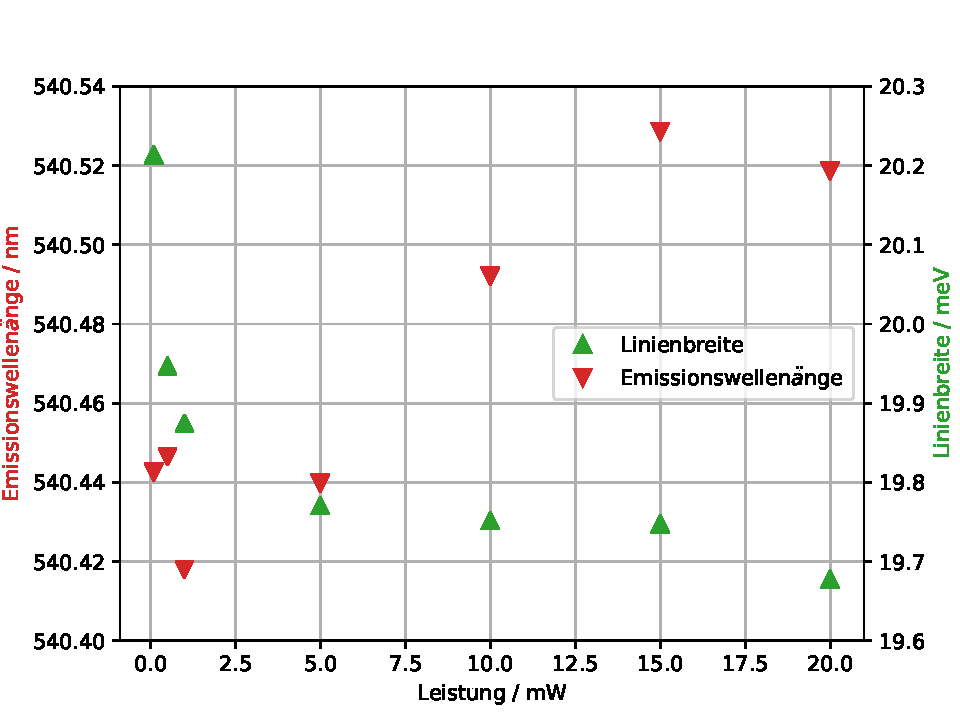
\includegraphics[width=0.6\textwidth]{Plots/aufgabe1c4_wl.pdf}
	\caption{Die Emissionswellenl\"{a}nge und Linienbreite der Probe 3 in Abh\"{a}ngigkeit der Laserleistung.}
	\label{abb:auf1c_ergebnisse}
\end{figure}
Zu sehen ist, dass die Linienbreite mit steigender Laserleistung abf\"{a}llt, wobei der Abfall zu h\"{o}heren Leistungen kleiner wird.
Die Linienbreite k\"{o}nnte sich hier einem S\"{a}ttigungswert ann\"{a}hern.
Im Gegensatz dazu ist bei dem Verlauf der Emissionswellenl\"{a}nge keine Tendenz zu erkennen.

\subsection{Abhängigkeit der Photolumineszenz von der Laserwellenlänge}
\label{sec:2}
In der zweiten Messreihe werden wieder alle drei Proben untersucht.
Diesmal werden die Proben mit unterschiedlichen Wellenl\"{a}ngen angeregt.
Verwendet werden Laser mit den Wellenl\"{a}nen $448 \,$nm, $518 \,$nm und $636 \,$nm.
Zum Vergleich ist in den folgenden PL-Spektren auch immer das PL-Spektrum der jeweiligen Probe aus dem ersten Aufgabenteil dargestellt, siehe Abbildung (\ref{abb:auf1a}).
In den Graphen (\ref{abb:auf2p1a}), (\ref{abb:auf2p2a}) und (\ref{abb:auf2p3a}) sind die Messwerte dargestellt.
Auch hier wurden, wie zuvor auch schon, die Messwerte f\"{u}r eine Messzeit von $1 \, s$ hochgerechnet, um die Spektren besser miteinander vergleichen zu k\"{o}nnen.
Zu sehen sind dabei jeweils in jedem Spektrum ein sehr schmaler Peak und ein breitere.
Der sehr schmale Peak wird Reflexionspeak genannt und stammt von dem Laser, mit dem die Probe angeregt wird.
Der breitere PL-Peak wird mit der Formel (\ref{form:gauss}) gefittet und ist jeweils in dem Graphen rechts daneben dargestellt.

In Abbildung (\ref{abb:auf2p1b}) ist zu sehen, dass die Nanokristalle der Probe 1 mit allen vier Wellenl\"{a}ngen angeregt werden k\"{o}nnen.
\begin{figure}[hbtp]
\centering
	\begin{subfigure}[t]{0.45\textwidth}
	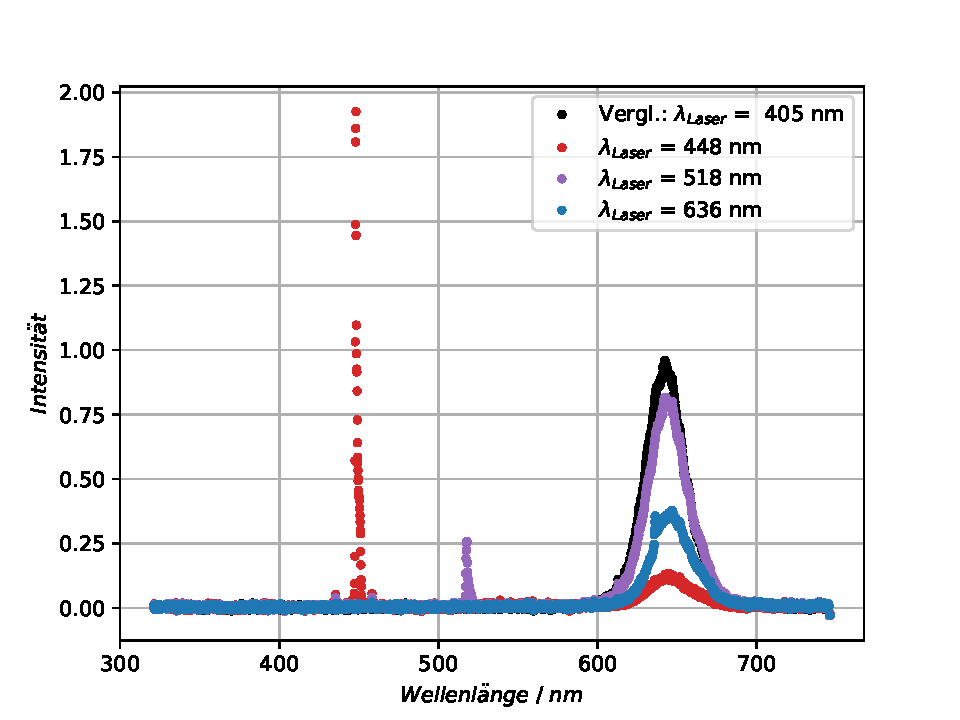
\includegraphics[width=\textwidth]{Plots/aufgabe2P1.pdf}
	\caption{PL-Spektren der Probe 1 mit unterschiedlicher Anregungswellenl\"{a}nge.}
	\label{abb:auf2p1a}
	\end{subfigure}
	~
	\begin{subfigure}[t]{0.45\textwidth}
	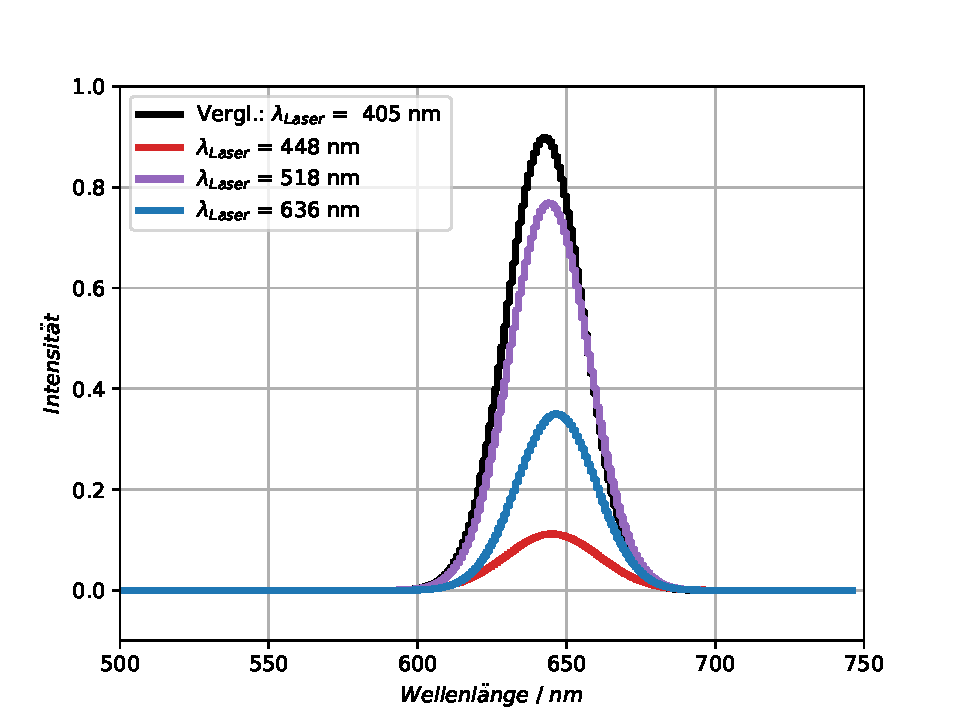
\includegraphics[width=\textwidth]{Plots/aufgabe2P1_fit_1s.pdf}
	\caption{Darstellung der Fits der PL-Peaks.}
	\label{abb:auf2p1b}
	\end{subfigure}
\caption{Messungen und Ergebnisse zur Probe 1.}
\label{abb:auf2P1}
\end{figure}
Die Messwerte, die aus den Fits abgelesen werden, sind in Tabelle (\ref{tab:auf2a}) notiert.
Hierbei steht die Abk\"{u}rzung Ref. f\"{u}r Reflexion und Emission wird mit Emi. bezeichnet.
Da sich der Reflexionspeak bei der Anregungswellenl\"{a}nge von $636 \, \text{nm}$ mit dem PL-Peak der Emission \"{u}berschneidet, k\"{o}nnen nur sehr wenige Messwerte zum Fitten des Reflexionspeak verwendet werden.
\begin{table}
	\centering
	\caption{Messergebnisse der Probe 1 zu Abbildung (\ref{abb:auf2P1})}
\begin{tabular}{|cccc|}
	\hline
	{$\lambda_{\text{Ref.}}$ / nm}	&	{Linienbreite Ref.}	&	{$\lambda_{\text{Emi.}}$ / nm}	&	{Linienbreite Emi.}	\\
	\hline
	448,32 & 0,69 & 645,31 & 18,47 \\
	517,99 & 0,85 & 644,23 & 15,73 \\
	636,51 & 1,48 & 646,68 & 15,67 \\
	\hline
	\end{tabular}
\label{tab:auf2a}
\end{table}

Im Vergleich zu Probe 1 sind die PL-Peaks der Probe 2 (siehe Abbildung (\ref{abb:auf2p2b})) etwas schmaler.
Hier ist nun auff\"{a}llig, dass f\"{u}r eine Anregung mit $636 \, \text{nm}$ keine Photolumineszenz auszumachen ist.
\begin{figure}[hbtp]
\centering
	\begin{subfigure}[t]{0.45\textwidth}
	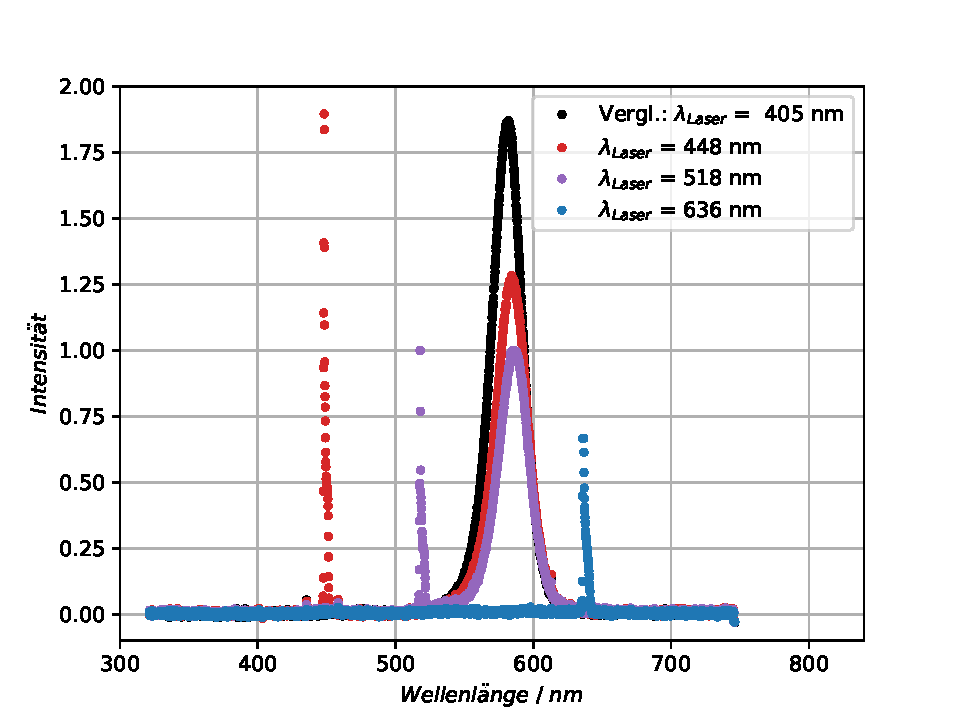
\includegraphics[width=\textwidth]{Plots/aufgabe2P2.pdf}
	\caption{PL-Spektren der Probe 2 mit unterschiedlicher Anregungswellenl\"{a}nge.}
	\label{abb:auf2p2a}
	\end{subfigure}
	~
	\begin{subfigure}[t]{0.45\textwidth}
	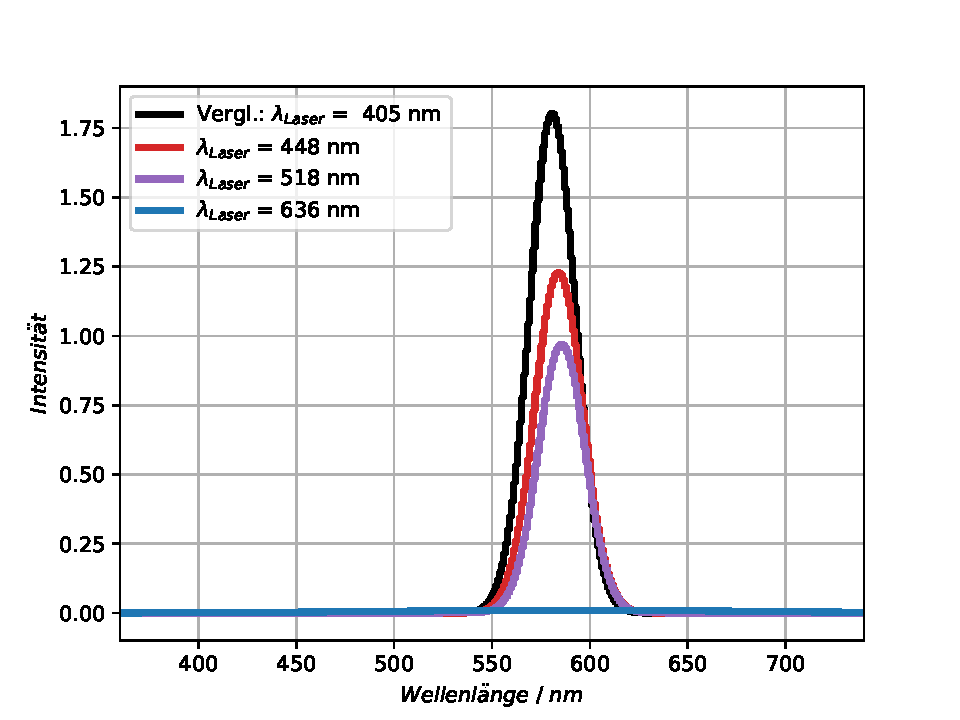
\includegraphics[width=\textwidth]{Plots/aufgabe2P2_fit_1s.pdf}
	\caption{Darstellung der Fits der PL-Peaks.}
	\label{abb:auf2p2b}
	\end{subfigure}
\caption{Messungen und Ergebnisse zur Probe 2.}
\label{abb:auf2P2}
\end{figure}
Werden die dazugeh\"{o}rigen Parameter aus Tabelle (\ref{tab:auf2b}) hinzugezogen, ist festzustellen, dass die Linienbreite eine ganze Gr\"{o}{\ss}enordnung gr\"{o}{\ss}er ist, als die der anderen PL-Peaks.
Die Messung k\"{o}nnte daher vernachl\"{a}ssigt werden, wird hier jedoch der Vollst\"{a}ndigkeit halber mit angegeben.
\begin{table}
	\centering
	\caption{Messergebnisse der Probe 2 zu Abbildung (\ref{abb:auf2P2})}
\begin{tabular}{|cccc|}
	\hline
	{$\lambda_{\text{Ref.}}$ / nm}	&	{Linienbreite Ref.}	&	{$\lambda_{\text{Emi.}}$ / nm}	&	{Linienbreite Emi.}	\\
	\hline
	448,50 & 0,93 & 584,02 & 14,44 \\
	518,19 & 1,05 & 585,65 & 14,09 \\
	636,97 & 1,62 & (589,88) & (109,10) \\
	\hline
	\end{tabular}
\label{tab:auf2b}
\end{table}

Zuletzt wird die Probe 3 mit unterschiedlichen Wellenl\"{a}ngen angeregt.
Wie schon bei der vorherigen Probe zu sehen, ist auch hier f\"{u}r eine Anregung mit $636 \, \text{nm}$ keine Photolumineszenz auszumachen.
\begin{figure}[hbtp]
\centering
	\begin{subfigure}[t]{0.45\textwidth}
	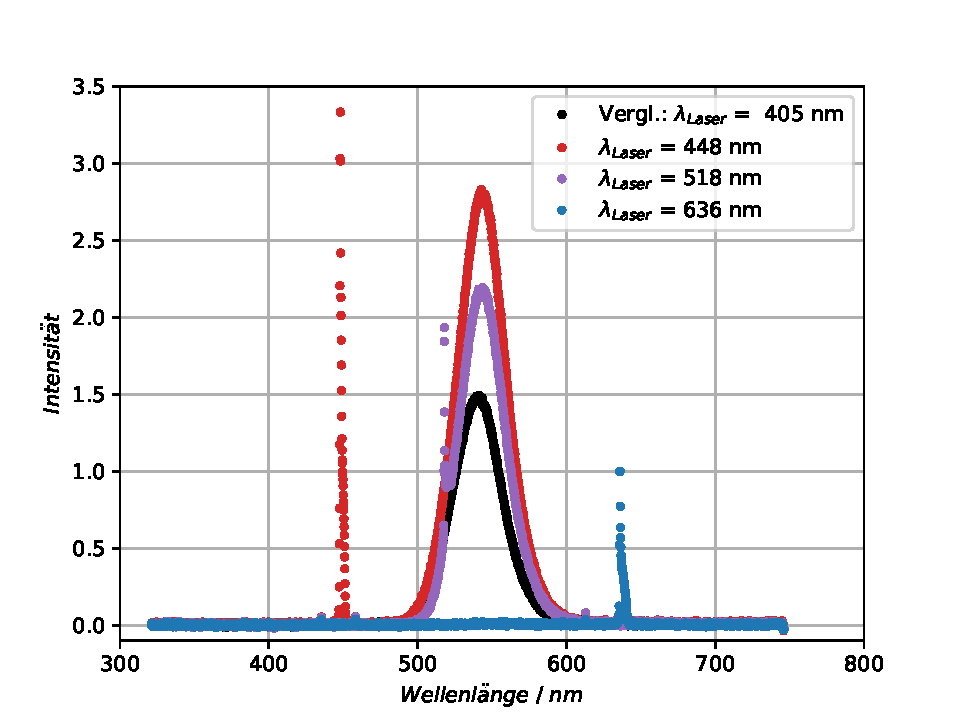
\includegraphics[width=\textwidth]{Plots/aufgabe2P3.pdf}
	\caption{PL-Spektren der Probe 3 mit unterschiedlicher Anregungswellenl\"{a}nge.}
	\label{abb:auf2p3a}
	\end{subfigure}
	~
	\begin{subfigure}[t]{0.45\textwidth}
	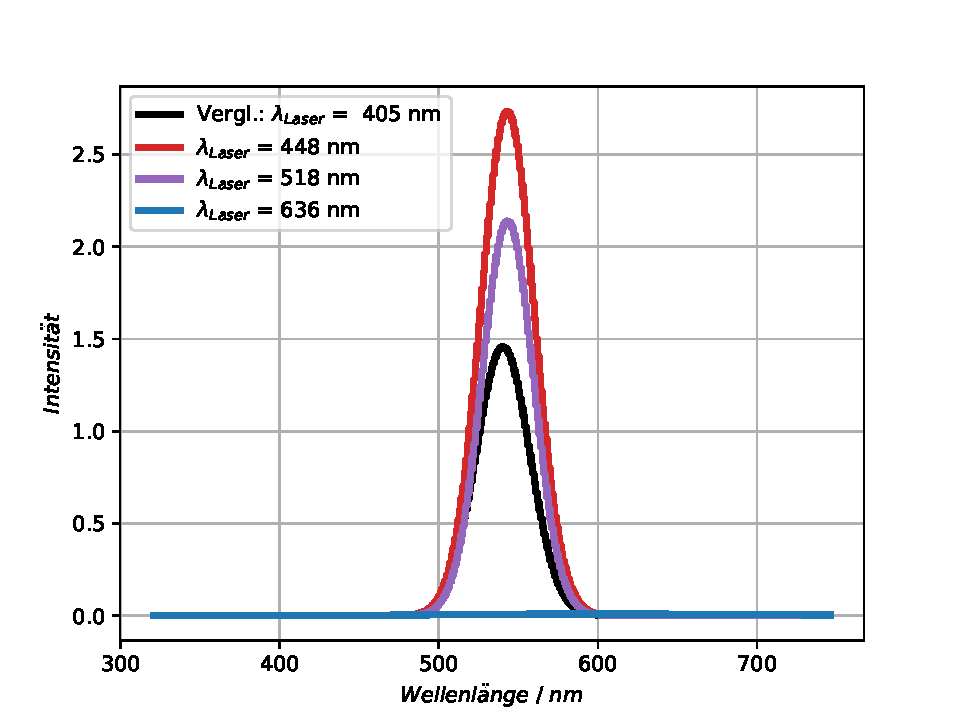
\includegraphics[width=\textwidth]{Plots/aufgabe2P3_fit_1s.pdf}
	\caption{Darstellung der Fits der PL-Peaks.}
	\label{abb:auf2p3b}
	\end{subfigure}
\caption{Messungen und Ergebnisse zur Probe 3.}
\label{abb:auf2P3}
\end{figure}
Auch hier k\"{o}nnen die Messdaten der Emission wieder vernachl\"{a}ssigt werden, da diese nicht aussagekr\"{a}ftig sind.
\begin{table}
	\centering
	\caption{Messergebnisse der Probe 3 zu Abbildung (\ref{abb:auf2P3})}
\begin{tabular}{|cccc|}
	\hline
	{$\lambda_{\text{Ref.}}$ / nm}	&	{Linienbreite Ref.}	&	{$\lambda_{\text{Emi.}}$ / nm}	&	{Linienbreite Emi.}	\\
	\hline
	448,36 & 0,82 & 543,13 & 19,79 \\
	517,96 & 0,20 & 543,34 & 19,05 \\
	636,58 & 1,42 & (610,95) & (100,88) \\
	\hline
	\end{tabular}
\label{tab:auf2c}
\end{table}

Bei einem Vergleich aller drei Proben ist festzustellen, das die PL-Peaks nur sehr wenig gegeneinander auf der x-Achse verschoben sind und lediglich die Intensit\"{a}ten stark unterschiedlich sind.
Zudem ist die Linienbreite der Emissionswellenl\"{a}nge deutlich h\"{o}her als die der Reflexionswellenl\"{a}nge.

\subsection{Linearer Polarisationsgrad von Flüssigkeiten (Bonus-Aufgabe)}
\label{sec:3}
Zuletzt wird der Polarisationsgrad einer Wein-Probe bestimmt.
Mit einem Laser der Wellenl\"{a}nge von $405 \, $nm wird diese angeregt.
Sowohl im Anregungspfad also auch im Detektionspfad wird die Polarisation variiert.
%mit dem lambda/2 plaettchen
Wie auch schon im vorherigen Aufgabenteil wird der sehr schmalen Peak in dem Spektrum durch eine Reflexion des Lasers hervorgerufen.
Dies ist beispielhaft in Abbildung (\ref{abb:auf3_P1_bsp}) zu sehen.
\begin{figure}[hbtp]
\centering
	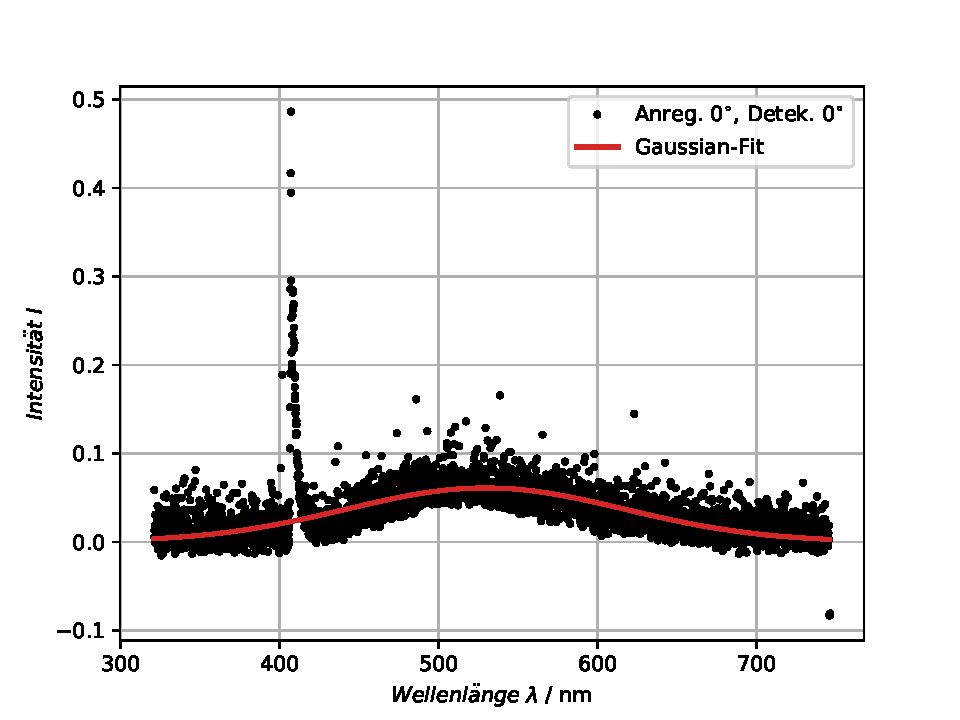
\includegraphics[width=0.6\textwidth]{Plots/aufgabe3_P1.pdf}
	\caption{Beispielhaft das vollst\"{a}ndige PL-Spektrum f\"{u}r die Messung mit $0^{\circ}$ im Anregungs- und Detektionspfad.}
	\label{abb:auf3_P1_bsp}
\end{figure}
Damit dieser Reflexionspeak den Fit nicht beeinflusst, wird im Folgenden nur das Intervall von $420 \,$nm bis $620 \,$nm betrachtet.
In Abbildung (\ref{abb:auf3}) sind die vier mit unterschiedlicher Polarisation aufgenommenen Spektren zu sehen.
\begin{figure}[hbtp]
\centering
	\begin{subfigure}[t]{0.45\textwidth}
	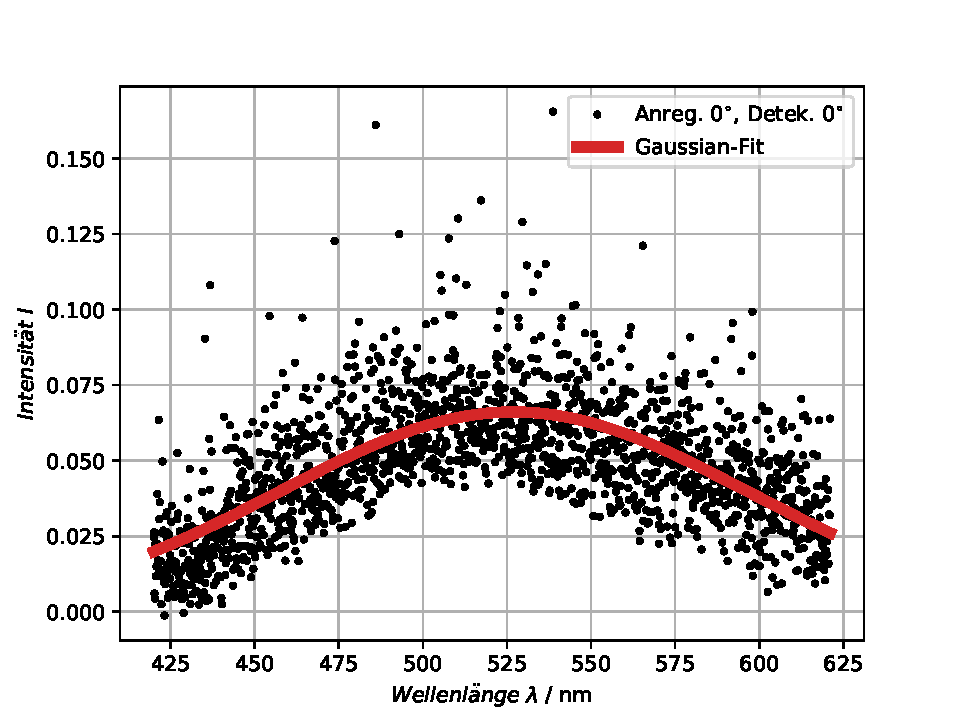
\includegraphics[width=\textwidth]{Plots/aufgabe3_P1_korrek.pdf}
	%\caption{}
	%\label{}
	\end{subfigure}
	%~
	\begin{subfigure}[t]{0.45\textwidth}
	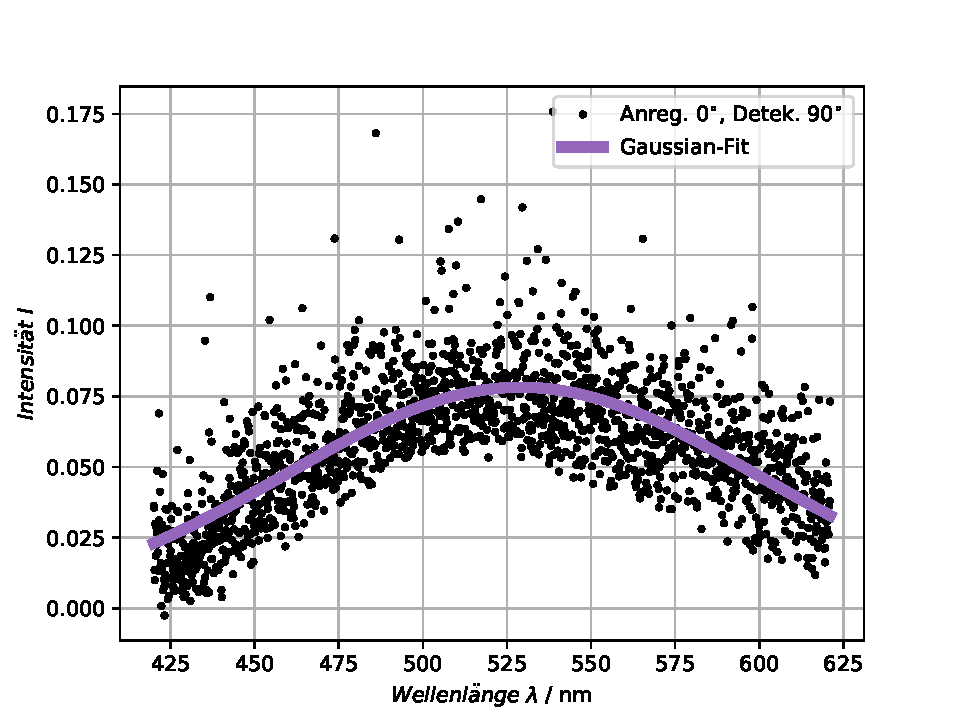
\includegraphics[width=\textwidth]{Plots/aufgabe3_P2_korrek.pdf}
	%\caption{.}
	%\label{}
	\end{subfigure}
	\\
	\begin{subfigure}[t]{0.45\textwidth}
	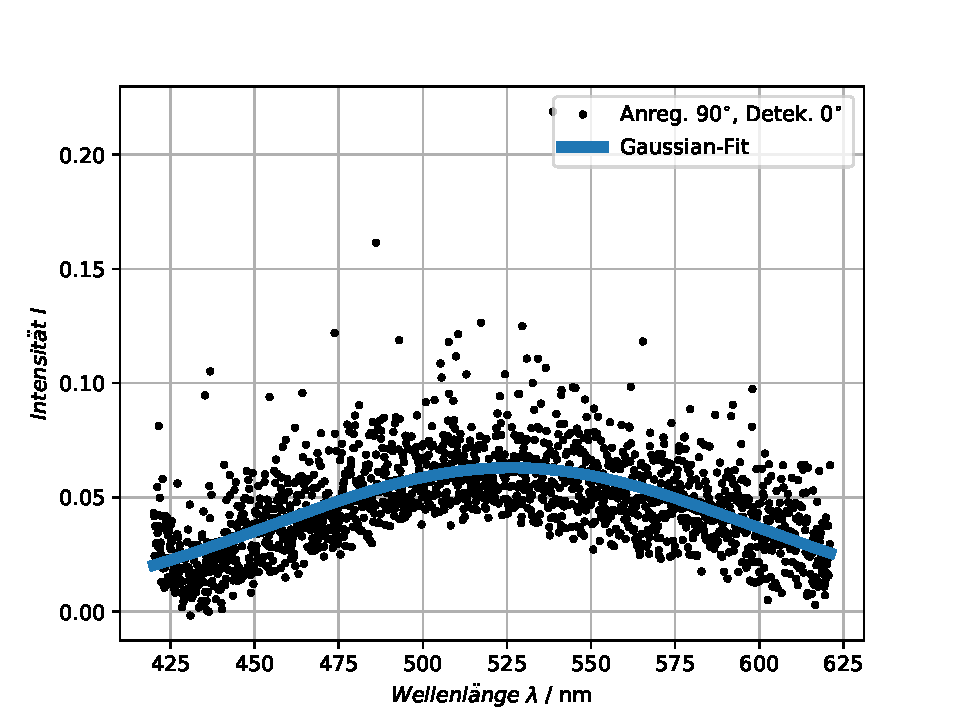
\includegraphics[width=\textwidth]{Plots/aufgabe3_P3_korrek.pdf}
	%\caption{}
	%\label{}
	\end{subfigure}
	%~
	\begin{subfigure}[t]{0.45\textwidth}
	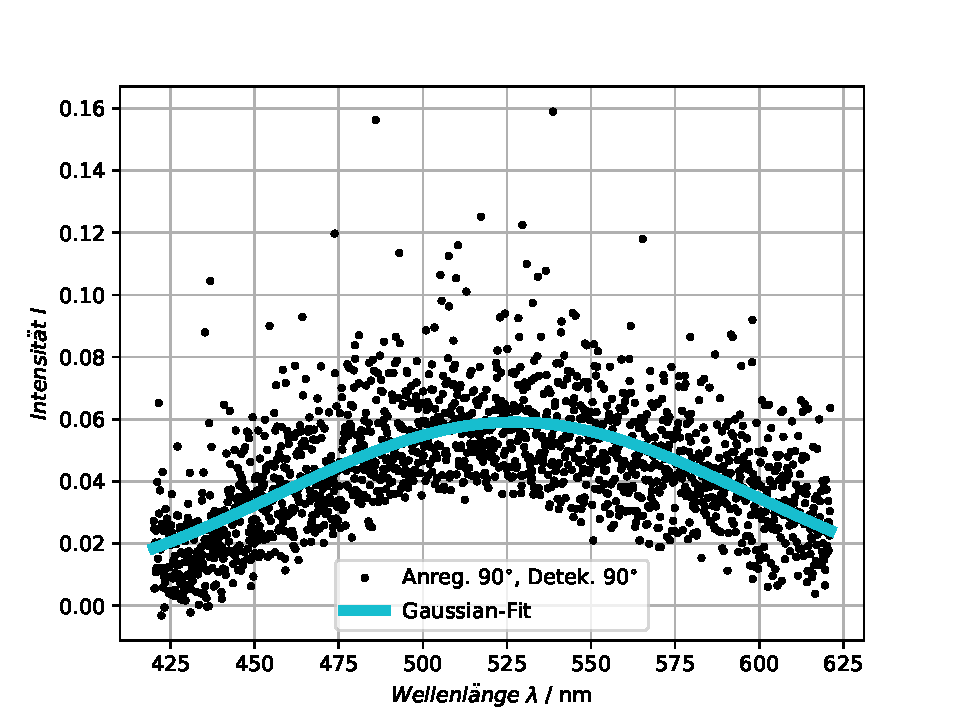
\includegraphics[width=\textwidth]{Plots/aufgabe3_P4_korrek.pdf}
	%\caption{.}
	%\label{}
	\end{subfigure}
\caption{Die PL-Spektren der Messungen von der Wein-Probe f\"{u}r verschiedene Polarisationspfade. Zu sehen ist jeweils nur das Intervall von (420 - 620)nm.}
\label{abb:auf3}
\end{figure}
Die PL-Peaks werden mit Formel (\ref{form:gauss}) gefittet.
F\"{u}r einen besseren Vergleich der vier Messungen miteinander sind die Fit-Kurven in Abbildung (\ref{abb:auf3_vergleich}) dargestellt.
\begin{figure}[hbtp]
\centering
	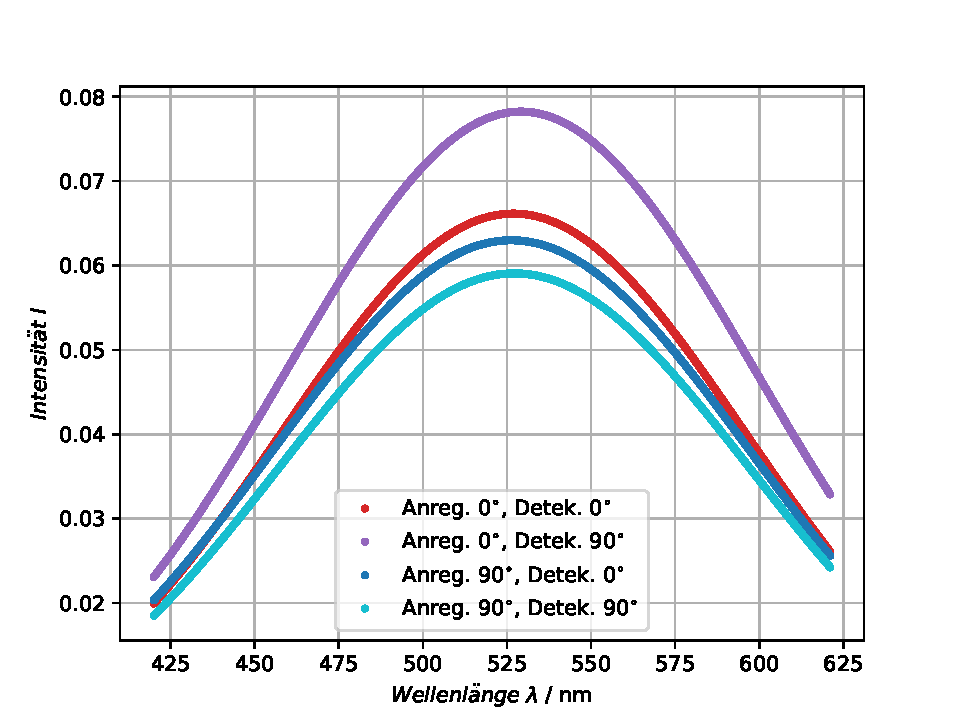
\includegraphics[width=0.6\textwidth]{Plots/aufgabe3_korrek.pdf}
	\caption{Die gefitteten Gau{\ss}-Kurven der vier gemessenen PL-Spektren im Vergleich.}
	\label{abb:auf3_vergleich}
\end{figure}
Die Position $x_0$ des Maximums der Gau{\ss}-Kurven ist untereinander ein wenig verschoben.
Auff\"{a}lliger sind die unterschiedlichen Intensit\"{a}ten der Maxima, welche in Tabelle (\ref{tab:auf3_vergleich}) notiert sind.
\begin{table}
\centering
\caption{Messwerte zu den gefitteten Gau{\ss}-Kurven.}
	\begin{tabular}{|rrcc|}
	\hline
	{Anregung} & {Detektion} & {Intensit\"{a}tsmaximum} &  \\
	\hline
	$0^{\circ}$ & $0^{\circ}$ & 0,0661 & 526,926\\
	$0^{\circ}$ & $90^{\circ}$ & 0,0782 & 529,136\\
	$90^{\circ}$ & $0^{\circ}$ & 0,0630 & 526,277\\
	$90^{\circ}$ & $90^{\circ}$ & 0,0591 & 527,174\\
	\hline
\end{tabular}
\label{tab:auf3_vergleich}
\end{table}
Aus den Intensit\"{a}tsmaxima wird mittels der Formel (\ref{form:polar}) der Polarisationsgrad berechnet.
\begin{equation}
	\text{Polarisationsgrad} = \frac{I_{PL,0^{\circ}} - I_{PL,90^{\circ}}}{I_{PL,0^{\circ}} + I_{PL,90^{\circ}}}
	\label{form:polar}
\end{equation}
F\"{u}r $0^{\circ}$ beziehungsweise $90^{\circ}$ im Anregungspfad ergeben sich damit die folgenden Werte des Polarisationsgrad.
\begin{align*}
	\text{P}_{0^{\circ}} &= 0,08377 \\
	\text{P}_{90^{\circ}} &= 0,03212 \\	
\end{align*}
